\documentclass[25pt, a0paper, landscape]{tikzposter}

% Preamble
\usepackage{tikz}
\usetikzlibrary{positioning}
\usetikzlibrary{arrows.meta,arrows}

\usepackage[backend=biber]{biblatex}


\usepackage{colortbl}

\usepackage[default,oldstyle,scale=0.95]{opensans} %% Alternatively
%% use the option 'defaultsans' instead of 'default' to replace the
%% sans serif font only.
\usepackage[T1]{fontenc}


% Layout

%% Title
\colorlet{backgroundcolor}{white}
\definetitlestyle{mytitle}{
	width=.99\linewidth,
}{}
\usetitlestyle{mytitle}
%%% Title wrap
\makeatletter
\def\title#1{\gdef\@title{\scalebox{\TP@titletextscale}{%
			\begin{minipage}[t]{\linewidth}
				#1
				\par
			\end{minipage}%
		}}}
\makeatother
%%% Title structure
\makeatletter
\renewcommand\TP@maketitle{%
	\begin{minipage}[t]{0.35\linewidth}
		\color{titlefgcolor}
		{\fontseries{sb}\selectfont \Huge {\@title}}
		{\large \@author \par}
		{\@institute \par}
	\end{minipage}%
	\hfill
	\begin{minipage}[t]{0.65\linewidth}
		~\\
		\hspace*{\fill}\@titlegraphic
	\end{minipage}
}
\makeatother

% Metadata
\title{Classifier-based latency estimation for covert attention ERP decoding}
\author{
	Arne Van Den Kerchove\textsuperscript{*,1,2},
	Hakim Si-Mohammed\textsuperscript{1},
	Marc Van Hulle\textsuperscript{2},
	François Cabestaing\textsuperscript{1}
}
\date{\today}
\institute{
	\textsuperscript{1}UMR CRIStAL, Univ. de Lille, Lille, France \\
	\textsuperscript{2}Lab for Neuro- and Psychophysiology, KU Leuven, Leuven, Belgium}
\titlegraphic{
	\includegraphics[height=8em]{figures/ulille.png}\hspace{1em}
	\includegraphics[height=8em]{figures/cristal.png}\hspace{1em}
	\includegraphics[height=8em]{figures/kul.png}
}
\addbibresource{references.bib}

\begin{document}
\maketitle
\begin{columns}
	\column{0.33}
	\block{1. Truly gaze-independent visual oddball interface}{

		\subsection*{Eye motor disability}

		\begin{minipage}{.48\linewidth}
			The BCI target population suffers from \textbf{eye motor disabilities}. This warrants the development of gaze-independent communication paradigms. While other active BCI modalities (auditory, somatosensory, ...) can work, visual paradigms exploiting \textbf{spatial attention} often yield the highest ITR~\cite{Riccio2012}.
		\end{minipage}%
		\hfill
		\begin{minipage}{.48\linewidth}
			\centering
			\textbf{Eye motor disabilities in patients}
			\bigskip

			\begin{tabular}{@{}|l|rrr|r|@{}}
				\hline
				         & ALS  & MS   & Stroke  &
				\cellcolor{yellow!25}\textbf{LiS}                                         \\ \hline
				Minor    & 50\% & 31\% & 40-70\% & \cellcolor{yellow!25}                  \\
				Severe   & 33\% & 3\%  & +       & \cellcolor{yellow!25}\color{black}98\% \\
				Complete & 17\% & -    & +       & \cellcolor{yellow!25}\color{black}2\%  \\ \hline
			\end{tabular}
		\end{minipage}


		\subsection*{Visual attention settings}
		%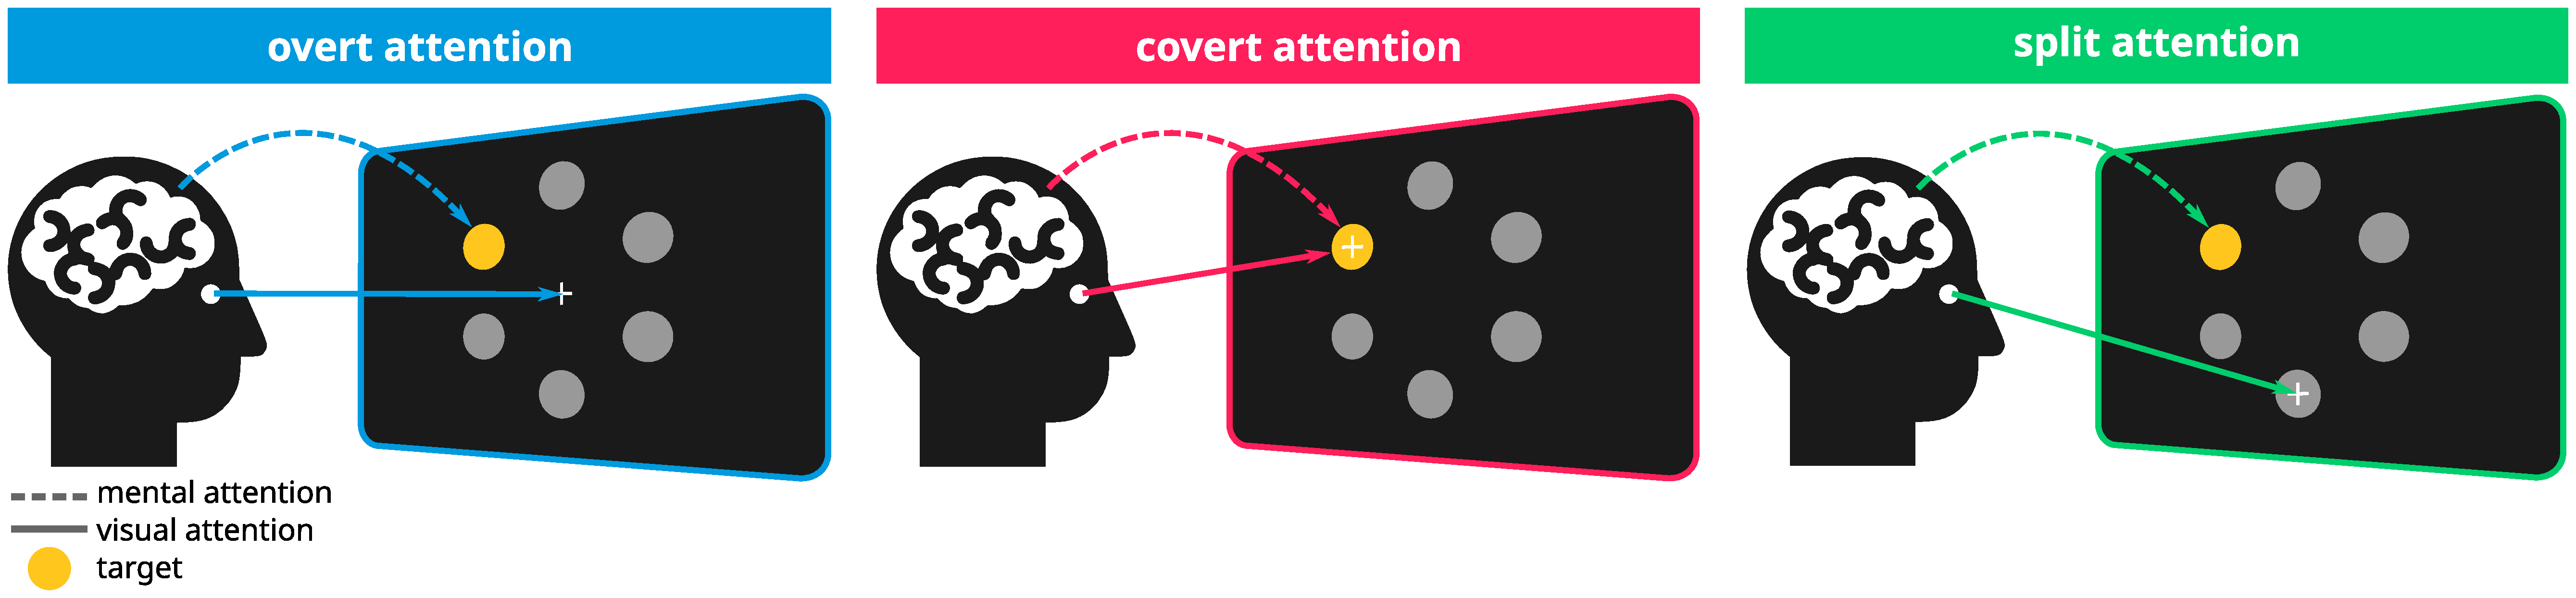
\includegraphics[width=\linewidth]{figures/attention_modes.eps}
		%Usually, a visual brain-computer interface is operated in \textbf{overt} attention mode, where the user directs their gaze to the intended target.
		%Patients with eye motor disabilities are not always able to comfortably perform overt attention.
		%Hence, \textbf{covert} attention paradigms have been designed where the user gazes at the center of the screen and selects targets in their visual periphery. Covert attention suffers from poor decoding performance, but this can be improved using \textbf{jitter correction}~\cite{Arico2014}. Further dissociating mental and visual attention

		\begin{minipage}{.48\linewidth}
			\includegraphics[width=\linewidth]{figures/attention_overt.pdf}
		\end{minipage}%
		\hfill%
		\begin{minipage}{.48\linewidth}
			Persons with full eye motor control can gaze at intended targets.
		\end{minipage}%
		\bigskip
		\bigskip

		\begin{minipage}{.48\linewidth}
			\includegraphics[width=\linewidth]{figures/attention_covert.pdf}
		\end{minipage}%
		\hfill%
		\begin{minipage}{.48\linewidth}
			Fixating the gaze at the center is a common solution, but this also requires a degree of eye motor control.
		\end{minipage}%
		\bigskip
		\bigskip

		\begin{minipage}{.48\linewidth}
			\includegraphics[width=\linewidth]{figures/attention_split.pdf}
		\end{minipage}%
		\hfill%
		\begin{minipage}{.48\linewidth}
			We design an interface that allows for the split attention conditions that can occurr in patients with involuntary eye movements.
		\end{minipage}%




		\subsection*{Experimental protocol}
		\includegraphics[width=\linewidth]{figures/paradigm.eps}
	}


	\column{0.33}
	\block{2. Novel ERP latency estimation procedure}{
		\cite{Sosulski2022}
		\textbf{Classifier-Based Latency Estimation (CBLE)}~\cite{Mowla2017}
		\begin{tikzfigure}
			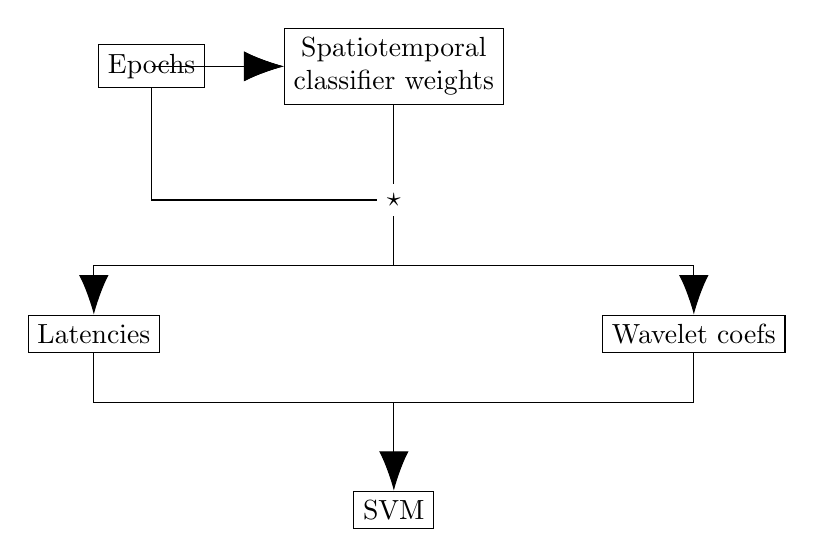
\begin{tikzpicture}
				\node[draw,align=center](class){Spatiotemporal \\ classifier weights};
				\node[below=of class,align=center](xcorr) {$\star$};
				\node[below=.5of xcorr](a1){};
				\node[draw,below=.5 of a1,align=center, xshift=-1.5in](latency) {Latencies};
				\node[draw,below=.5 of a1,align=center,xshift=1.5in](wav) {Wavelet coefs};
				\node[draw,left=of class,align=center](epochs) {Epochs};
				\node[below=.5of latency, xshift=1.5in](a2){};
				\node[draw, below= of a2,align=center](svm) {SVM};

				\draw[-{Latex[length=.2in]}] (epochs) to (class);
				\draw[-{Latex[length=5mm]}] (epochs) |- (class);
				\draw (class) to (xcorr);
				\draw (xcorr) to (a1.center);
				\draw[-{Latex[length=5mm]}] (a1.center) -| (latency);
				\draw[-{Latex[length=5mm]}] (a1.center) -| (wav);
				\draw (epochs) |- (xcorr);
				\draw (latency) |- (a2.center);
				\draw (wav) |- (a2.center);
				\draw[-{Latex[length=5mm]}] (a2.center)  to (svm);
			\end{tikzpicture}


		\end{tikzfigure}
		\bigskip

		\textbf{Woody Classifier-Based Latency Estimation (wCBLE)}
		\begin{tikzfigure}
			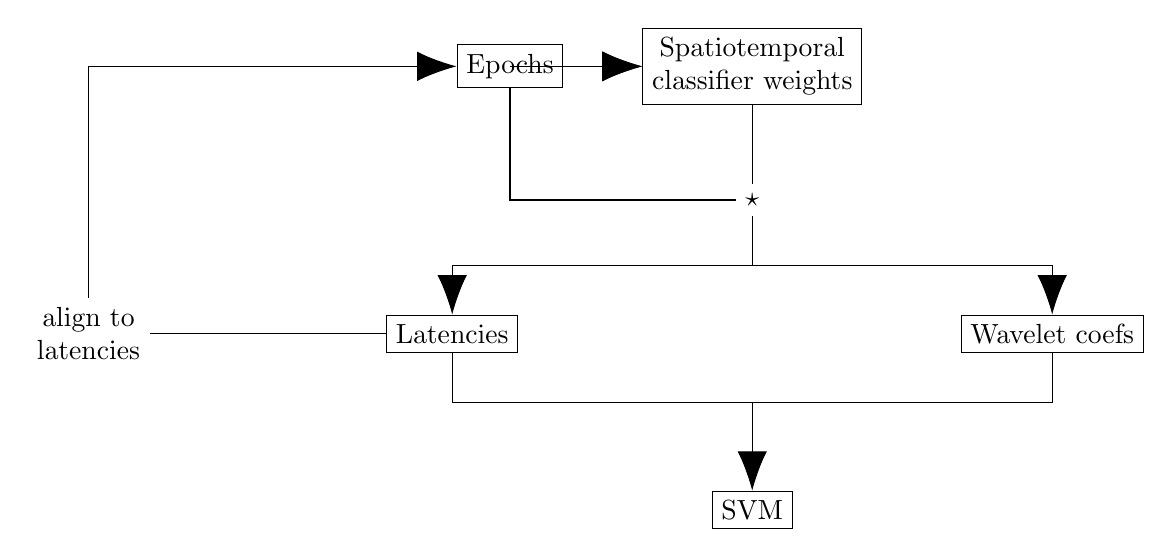
\begin{tikzpicture}
				\node[draw,align=center](class){Spatiotemporal \\ classifier weights};
				\node[below=of class,align=center](xcorr) {$\star$};
				\node[below=.5of xcorr](a1){};
				\node[draw,below=.5 of a1,align=center, xshift=-1.5in](latency) {Latencies};
				\node[draw,below=.5 of a1,align=center,xshift=1.5in](wav) {Wavelet coefs};
				\node[draw,left=of class,align=center](epochs) {Epochs};
				\node[left=3 of latency, align=center](align){align to \\ latencies};
				\node[below=.5of latency, xshift=1.5in](a2){};
				\node[draw, below= of a2,align=center](svm) {SVM};
				\node[left=.5of epochs](a3){};

				\draw[-{Latex[length=.2in]}] (epochs) to (class);
				\draw[-{Latex[length=5mm]}] (epochs) |- (class);
				\draw (class) to (xcorr);
				\draw (xcorr) to (a1.center);
				\draw[-{Latex[length=5mm]}] (a1.center) -| (latency);
				\draw[-{Latex[length=5mm]}] (a1.center) -| (wav);
				\draw (epochs) |- (xcorr);
				\draw (latency) |- (a2.center);
				\draw (wav) |- (a2.center);
				\draw[-{Latex[length=5mm]}] (a2.center)  to (svm);
				\draw (latency)  to (align);
				\draw (align.north)  |- (a3.center);
				\draw[-{Latex[length=5mm]}] (a3.center)  to (epochs);
			\end{tikzpicture}


		\end{tikzfigure}

		\bigskip
		\textbf{Convergence}

		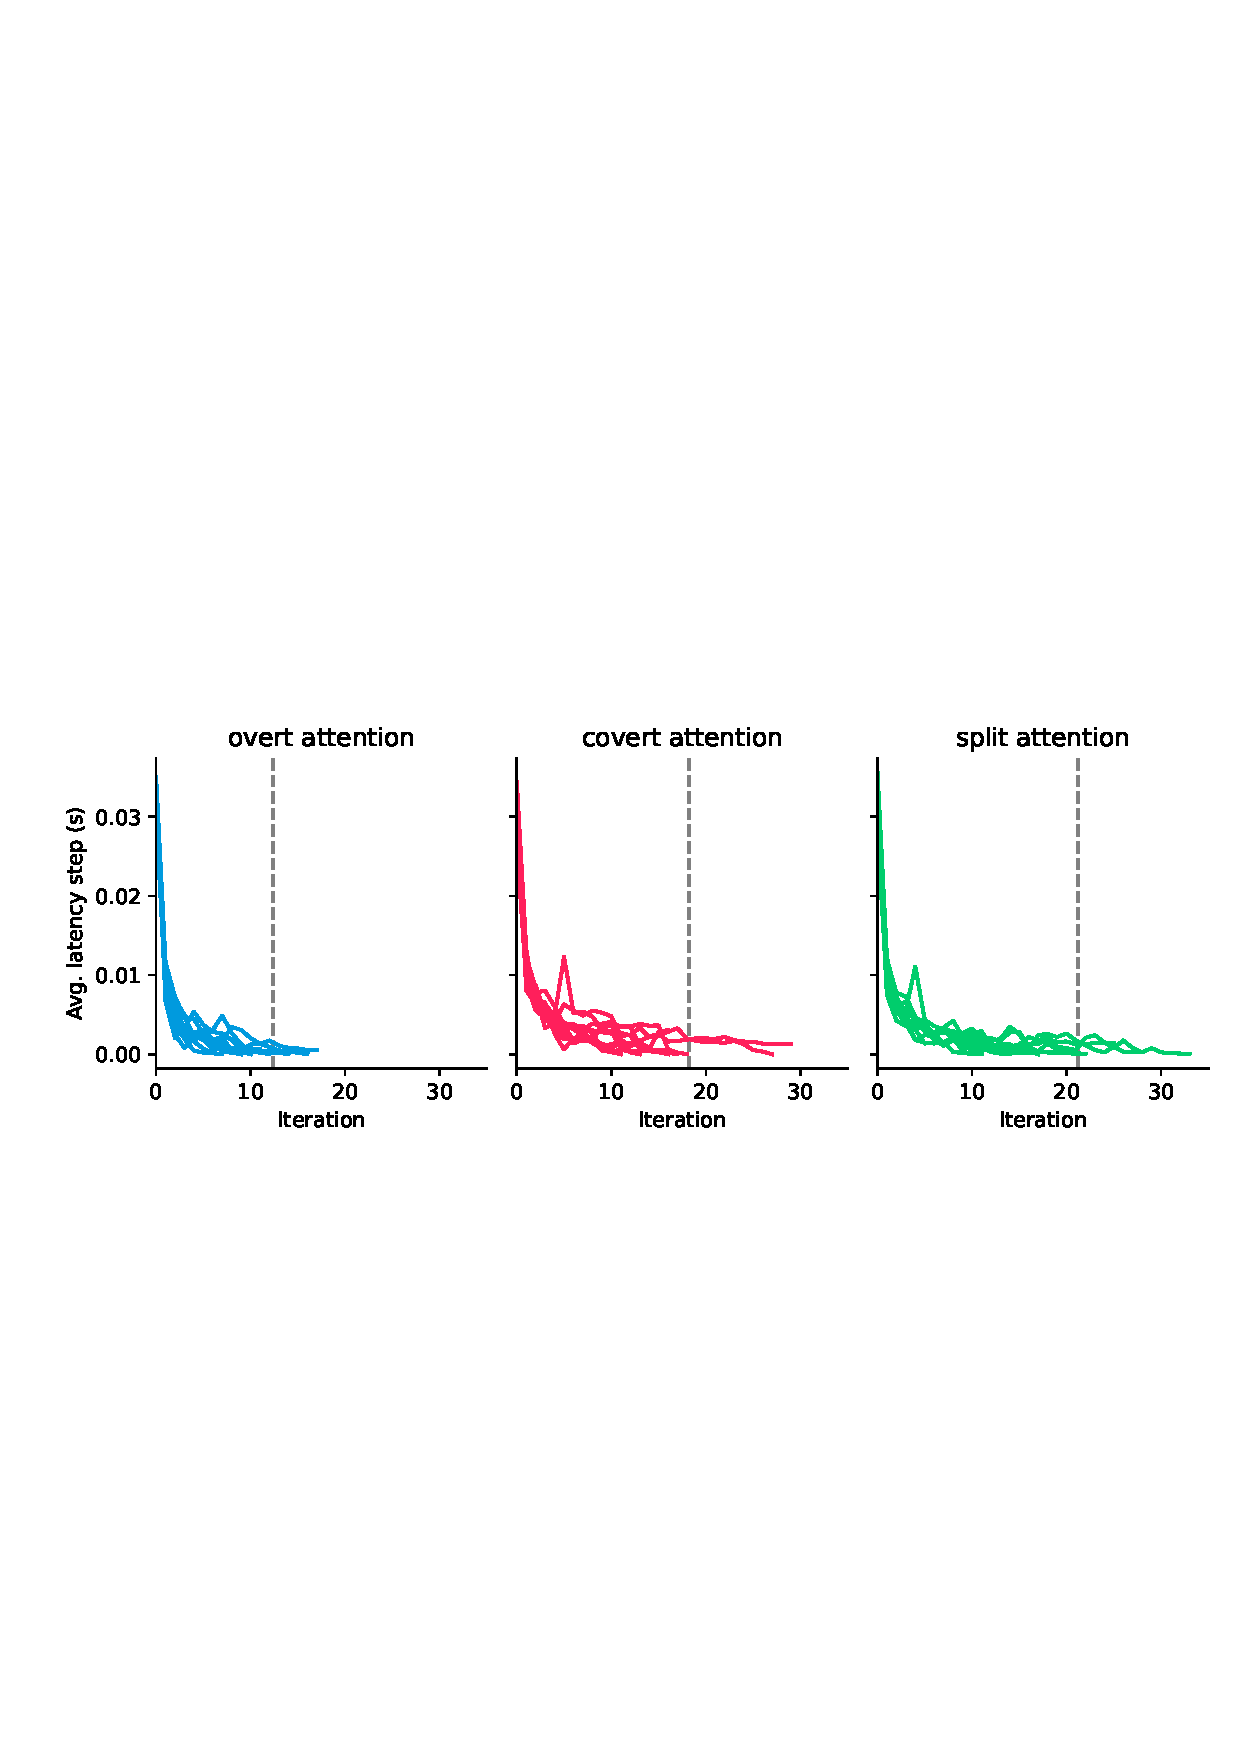
\includegraphics[width=\linewidth]{figures/convergence.png}

		\bigskip
		\textbf{Alignment}
	}

	\column{0.33}
	\block{3. Improvement in covert attention decoding}{
		\begin{enumerate}
			\item Band-pass .5 to 32Hz
			\item Resample to 64Hz
			\item ICA Eye artifact rejection
			\item Remove bad trials according to eye-tracker
			\item Subtract non-target average
		\end{enumerate}

		\includegraphics[width=.5\linewidth]{figures/classification_results_diff.png}

		\includegraphics[width=\linewidth]{figures/classification_results_rel.eps}
	}
	\block{Conclusion}{
		\begin{enumerate}
			\item
			\item
			\item
		\end{enumerate}
	}
	\block{References}{
		\printbibliography[heading=none]
	}
\end{columns}

\end{document}
